\section{Theory}
	Going through the theory in the book \textit{Sensation and perception}, to categorize the different depth cues a tree was made, and to give structure to my report, I remade a copy of it as seen \autoref{fig:depthCues}, and I will utilize this for presenting my findings and answering the topic questions. The order in which I will present the different depth cues will also be much akin of that found in the book.
	\begin{figure}[H]
		\centering
		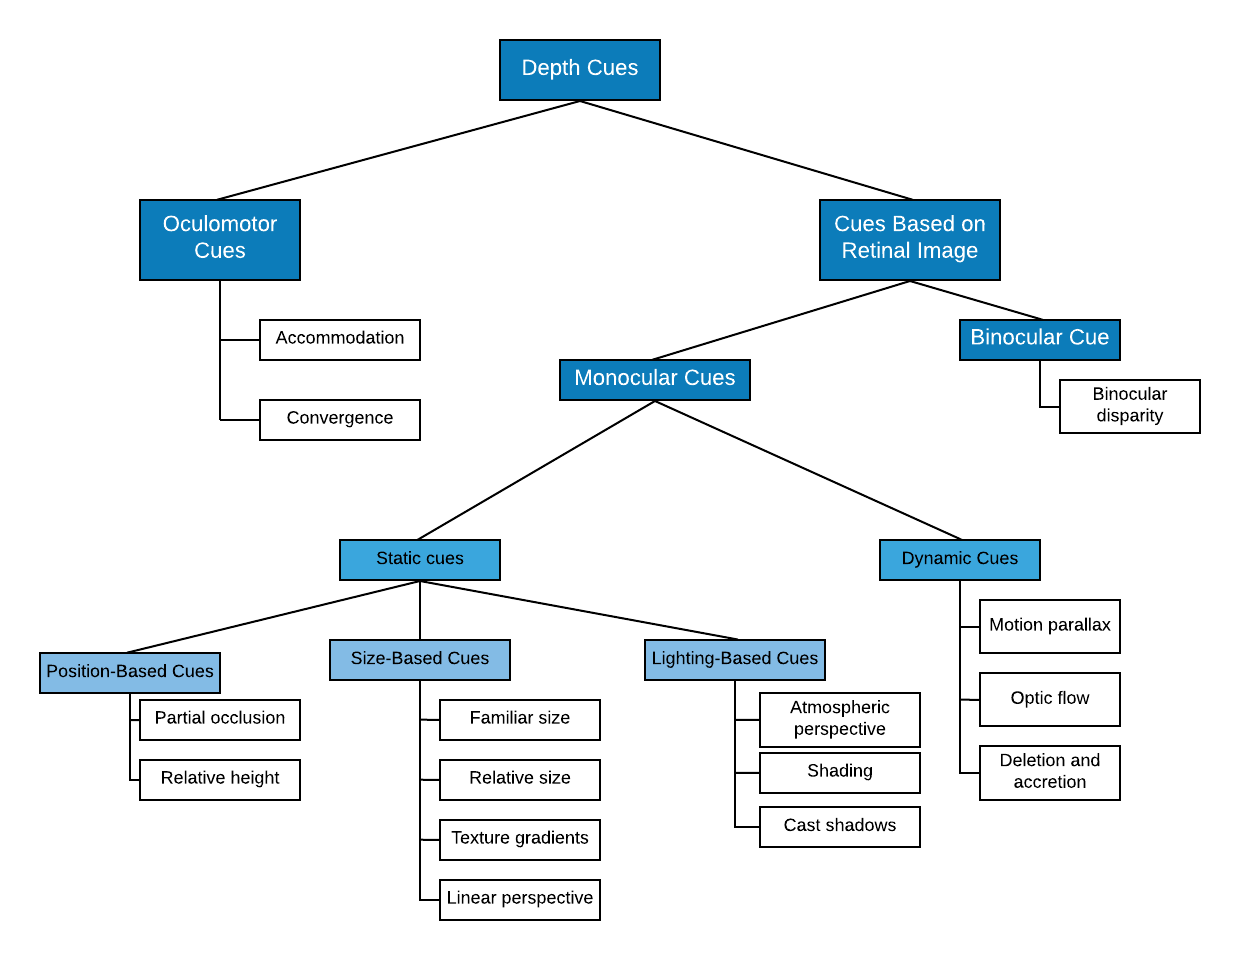
\includegraphics[width=1\linewidth]{figure/depthcues}
		\caption{All the depth cues from the book, Sensation and Perception\citep{sensationPerception}, the figure was made as a copy from the figure on page 195.}
		\label{fig:depthCues}
	\end{figure}
	\subsection{Oculomotor depth cues}
		This section deals with how the two different sets of muscles in the eyes, gives depth cues on our surrounding world. The two sets of muscles are specifically those that manage and control the position of eyes; which direction they point and the likes, and those that manage the shape of the lens in the eye; changing focus to adjust for distance.
		\subsubsection{Accommodation}
			Whenever you look out on the world around you, there are objects which differ in distance from your eyes, and because your eyes uses, among others, a lens to direct the light into your retina, objects that are farther away than what your lens is shaped to focus on, would seem blurry, if not for our ciliary muscles. These muscles contract and and relax our lens, in turn focusing the light entering our eyes. The whole system works automatically due to our autonomic nervous system \citep{sensationPerception}. Objects farther away require a more flat lens, and object closer to your eyes, require a more round shaped lens as seen in \autoref{fig:accommodation}.
			\begin{figure}[H]
				\centering
				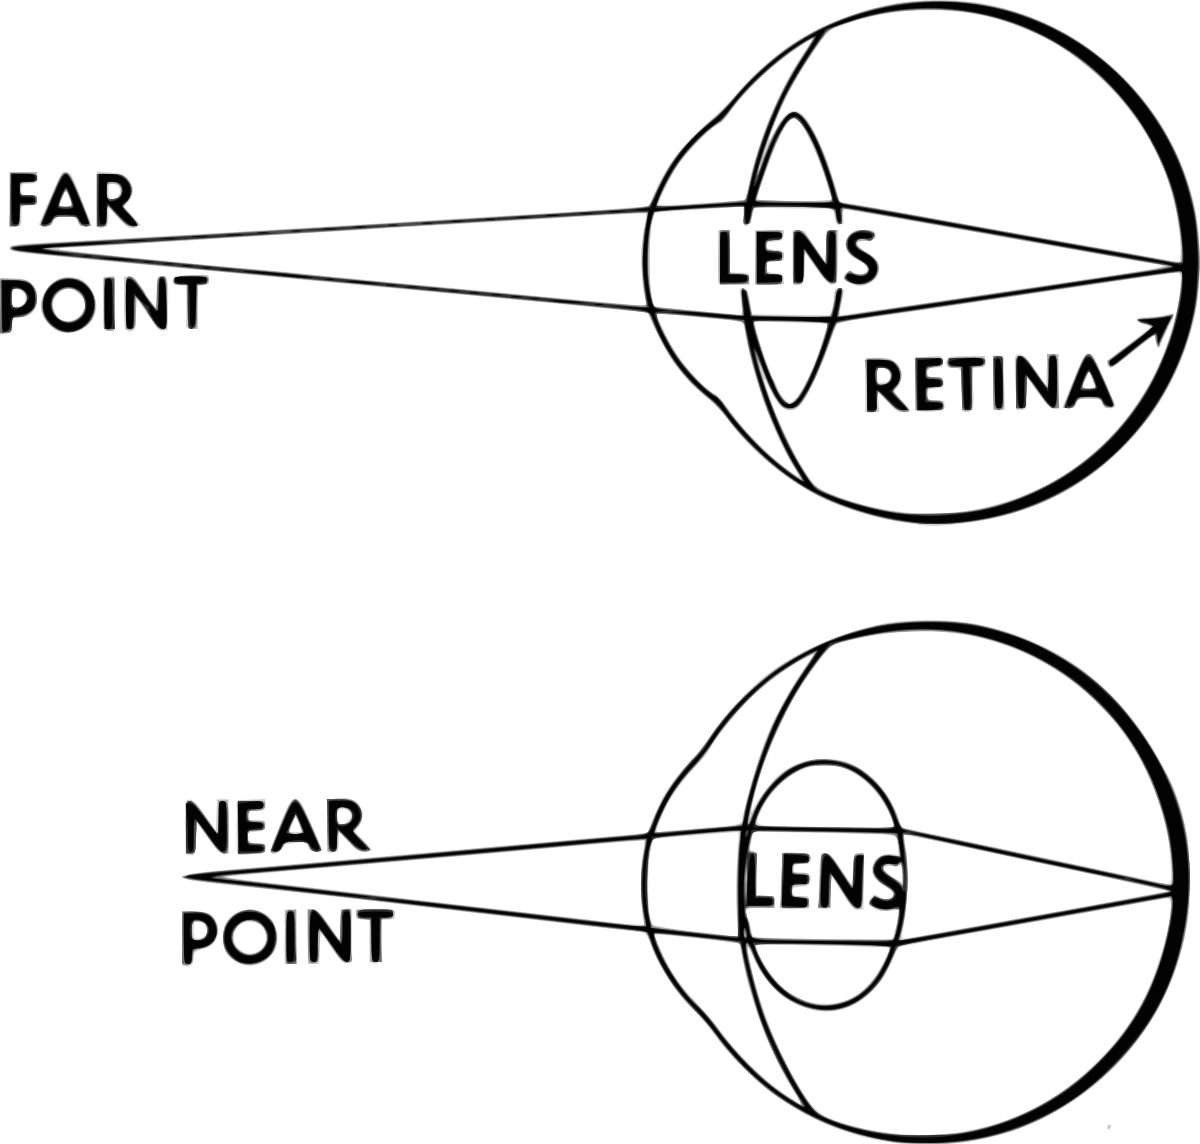
\includegraphics[width=0.5\linewidth]{figure/accommodation.png}
				\caption{Figure taken from \citep{wikiaccommodation} that demonstrates the different lens shapes depending on the distance of the object looked at.}
				\label{fig:accommodation}
			\end{figure}
			
			Mark Mon-Williams \& James R. Tresilian did undergo research into the depth information that is gained from  accommodation, and the information gotten from this cue can be very imprecise, and can only really provide depth information on objects at no more than 2 m away \citep{accommodation}.
		\subsubsection{Convergence}
			When you are looking at a dog far away, like 150 m, your eyes are positioned so that your sight is looking straight ahead of your head, to look directly at the dog. The angle between your lines of sight, are close to zero\textdegree, in turn almost parallel. If that same object moved closer, like 1 m away, your eyes would start \textit{converging} on each other, turn inward \citep{sensationPerception}. If the dog was 1 m away from your eyes the angle between your lines of sight, would be about 3.5\textdegree\citep{sensationPerception}. 
	\subsection{Monocular Depth cues}
		The most significant depth cues we get from our eyes, are the ones that are gotten from the retinal image \citep{sensationPerception}. These cues cover a wide range of scenarios, and gives information in most situations we humans find ourselves in. This section will cover the depth cues that are gotten from our retinal image, requiring only one eye.
		\subsubsection{Static cues}
			The first cues that will be covered in this section are the static cues, these cues require no movement in the scene that we are looking at, be it a picture, a painting, or a still real scene.
			%Position
			\paragraph{Partial Occlusion}
				One cue that gives much depth information of a scene, is partial occlusion, the fact that objects in 3D space can partially cover each other from our perspective. This is easily demonstratable by looking at \autoref{fig:partialocclusion}, which gives a straight forward idea of partial occlusion. Due to the green square occluding part of the purple square, we assume that the green square is in front of the purple one. Likewise with the red square, which is partially occluded by the purple, which in turn we assume means it is farther away than the purple on, so due to the depth cues inferred from this image, the purple square is between the green and the red, in terms of distance.
				\begin{figure}[H]
					\centering
					
\includegraphics[width=0.4\linewidth]{figure/partialocclusion}
					\caption{Figure demonstrating partial occlusion, the green square looks to be in front of the purple square, which looks to be in front of the red square, which infers depth in a 2D image.}
					\label{fig:partialocclusion}
				\end{figure}
				The pitfall of this cue, specifically when looking at 2D images like \autoref{fig:partialocclusion}, is that the red and purple just might have a cutout in which the green fit perfectly into the purple, and the purple fit directly into the red square. This is however quite unlikely, but it demonstrates that the cue works a lot of off the assumption that the squares are overlapping each other, and not simply fitting together perfectly.
			\paragraph{Relative Height}
				The position of objects in relation to your eye level. Objects closer to the horizon or eye level seem farther away, while objects further from that level, seems closer \citep{relativeHeight}. Looking at \autoref{fig:relativeHeight}, the green square that is closest to the horizon look to be further away than the green square the is further away from the horizon. 
				\begin{figure}[H]
					\centering
					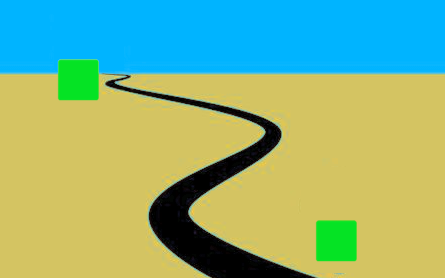
\includegraphics[width=0.6\linewidth]{figure/relativeHeight}
					\caption{Figure demonstrating relative height; the green square that is closer to the horizon looks to be farther away than the one that is farther from the horizon.}
					\label{fig:relativeHeight}
				\end{figure}
				Suppose you are looking into a room, say the living room, there's a television, a ceiling lamp and a sofa. When looking straight ahead you see the television at your eye level. The ceiling lamp can be seen above the television, and the sofa can be seen below. The ceiling lamp and sofa, looks to be closer to you, while the television looks to be the farthest from you, that is relative height.
			%Size
			\paragraph{Familiar Size}
				When we see plate with a piece of lasagna on it, we have an idea of the size a normal plate has, and having eaten lasagna before, we have an assumption of the size of that piece, in relation the plate it is on. We base the information on knowing the general size of a plate, and lasagna, it is something we are familiar with, \textbf{\textit{familiar size}}.\\\\ In a nonfood related scenario, imagine a golf ball and basketball, we have a expectation to the size of both, at least to the size ratio, the basketball usually being bigger than the golf ball. When looking at \autoref{fig:familiarSize}, (a) shows the golf ball next to the basketball, and the familiar sizes gives the cue that the balls are next to each other in 3D space. When looking at (b) though, the golf ball now looks to be same size on retinal image, as the basketball, we assume that the golf ball is normal golf ball size, and simply most be closer to the our eyes, than the basketball.
				\begin{figure}[H]
					\centering
					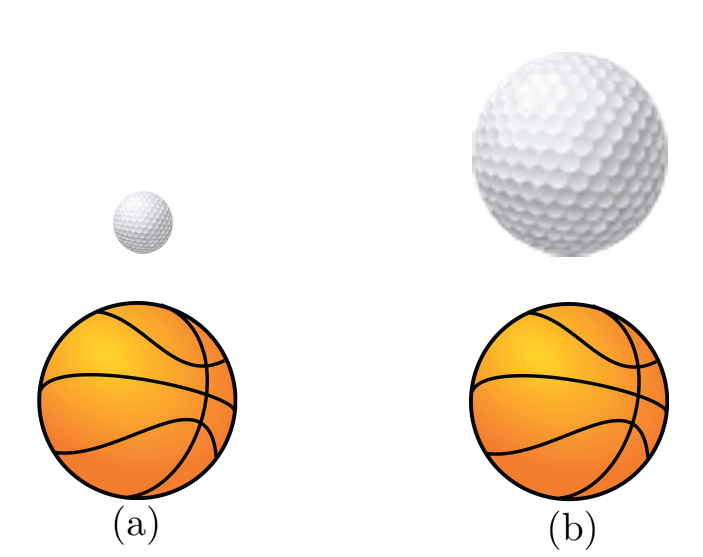
\includegraphics[width=0.5\linewidth]{figure/familiarSize}
					\caption{Figure demonstrating familiar sizes, expectations of size, due to having familiarity with golf balls, and basketballs. (a) Normal relationship between the balls (b) Golf ball seems to be the same size as the basketball, this must mean that golf ball is closer than the basketball, or a small basketball/big golf ball.}
					\label{fig:familiarSize}
				\end{figure}
				The pitfall with this depth cue, is that the golf ball in (b) might simply be basketball sized, and actually is right next to the basketball in 3D space. Or the basketball might be golf ball sized, but both of these scenarios are highly unlikely however, as we humans simply expect and assume that conditions are familiar and rely on the the depth cues we get.
			\paragraph{Relative Size}
				Relative size works a lot like familiar size, by using the relative size of objects to infer depth information, but doesn't require the viewed objects to be familiar. Instead it focuses on the relative size of the objects in the scene, so if you had 6 pomelos next to each other, even though you haven't seen a pomelo before, we can still extract depth information from their relative size to each other, so if one pomelo was gradually smaller than the other, we can assume that it is either a very small pomelo, or simply further away than the others.
			\paragraph{Texture Gradients}
				Looking at \autoref{fig:textureGradient} the texture of the stone tiles gets smaller the further away it is. This cue is very reliable, because most surfaces and objects have a texture, and hence can potentially produce this effect when viewed.
				\begin{figure}[H]
					\centering
					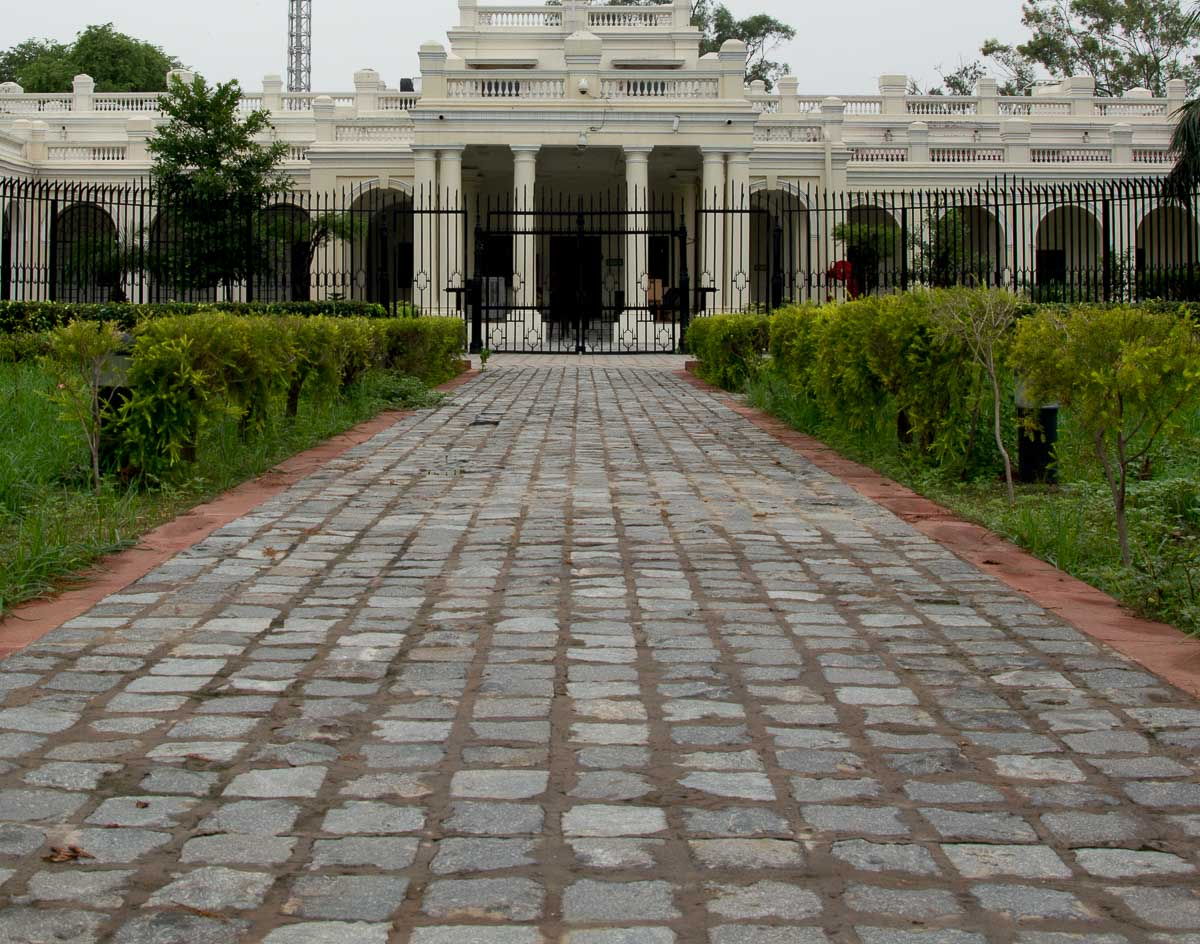
\includegraphics[width=0.6\linewidth]{figure/gradient}
					\caption{Texture gradients are like normal gradients, but has to do with the texture getting smaller the farther it is from your eyes, thus behaving like a color gradient, but for texture and its size. [Copyright: Ashish Bhart]}
					\label{fig:textureGradient}
				\end{figure}
			\paragraph{Linear Perspective}
				The scene in \autoref{fig:linearPerspective}, very well demonstrates how linear perspective infers depth. The road keeps going out into the horizon, and the road borders will slowly converge unto each other until they are nothing but a spot on the horizon.
				\begin{figure}[H]
					\centering
					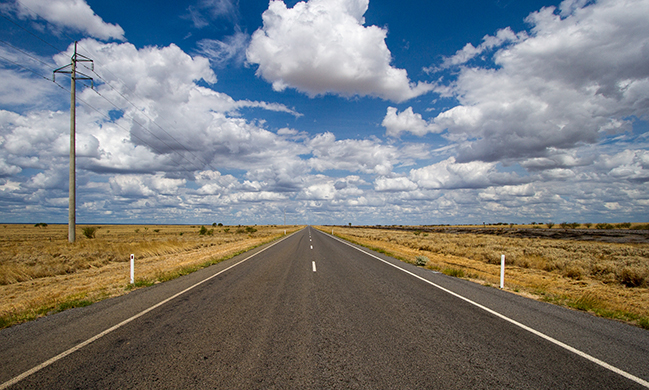
\includegraphics[width=0.8\linewidth]{figure/linear}
					\caption{Linear perspective behaves a bit like texture gradients, but instead focuses on parallel lines in the scenes we see. The lines of the road slowly converge on each other the farther away they get, inferring depth and thus distance. [Copyright: Marc Dalmulder]}
					\label{fig:linearPerspective}
				\end{figure}
			%Lighting
			\paragraph{Atmospheric Perspective}
				Due to the dust and other particles in the air, the light waves that are coming from the most distant mountains seen in \autoref{fig:atmosphericPerspective} will have a slightly bluish tint, due to the dark wavelengths that the mountains give \citep{atmoshpericPerspective}. Lighter objects will give a more reddish tint \citep{atmoshpericPerspective}. 
				\begin{figure}[H]
					\centering
					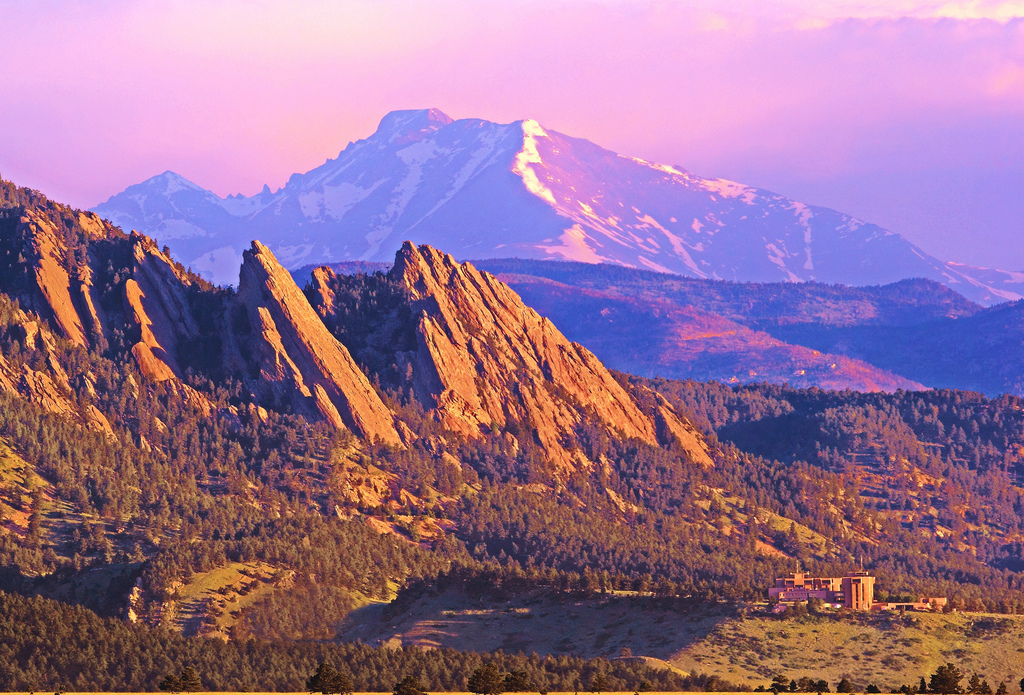
\includegraphics[width=0.8\linewidth]{figure/atmosphericperspective}
					\caption{Image demonstrating how atmospheric perspective works, looking at the blue-ish tint coming from the distant mountains, they seem very far away, because of the way the dark colors coming from them gets scattered through the air and dust, resulting in the blue-ish color, and slightly non-distinct outlines.}
					\label{fig:atmosphericPerspective}
				\end{figure}
			\paragraph{Shading}
				One of the many constants in human existence, is the sun above our heads. This leads to some assumptions and expectations when it comes to the shading of objects in our life. We infer depth from how a object is shaded, as can be seen in \autoref{fig:shading}. The left circle set looks to be illuminated from the top, and looks to \textit{pop out} of the image, compared to the right side, where the circles look to be illuminated from the bottom, making them look like they are concave.
				\begin{figure}[H]
					\centering
					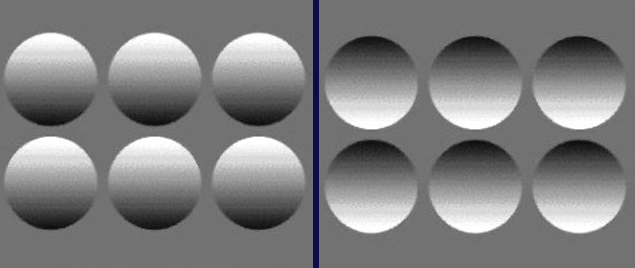
\includegraphics[width=0.8\linewidth]{figure/shading}
					\caption{Two sets of circles demonstrating how shading changes how the depth is inferred from the picture. The left side circles seem like they are raised from the picture, while the right set looks like they are indented into the image.}
					\label{fig:shading}
				\end{figure}
			\paragraph{Cast shadow}
				In a normal day we see shadows all the time, and they give us indication of depth. All people have a shadow, and if it is at their feet, we know that person isn't defying gravity. When an object is lying on a table, it casts a shadow onto it, so we know the it in fact is lying on the table. Three cubes can be seen in \autoref{fig:castShadow}, all with a fake shadow applied to them, giving a sense of depth in the image, when in reality there is none.
				\begin{figure}[H]
					\centering
					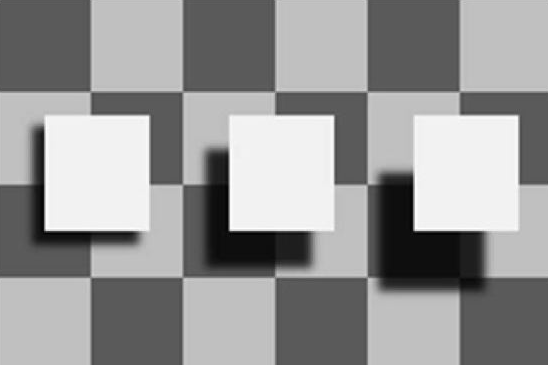
\includegraphics[width=0.5\linewidth]{figure/castShadow}
					\caption{This is a 2D image, with 3 cubes, these cubes are right next to each other, yet it seem like the one to the far right is above the other, and the middle cube is above the left most one. This is due to the fact that these cubes have been given a \textit{shadow}, a same sized black blurry version displaced \textit{beneath} them. The further the shadow is displaced the higher it seem the cube is flying. [Copyright: David Heeger]}
					\label{fig:castShadow}
				\end{figure}
		\subsubsection{Dynamic cues}
			The last section dealt with cues that we humans can infer depth information from still scenes, images and the like. This section deals with the depth cues that require motion to provide any information.
			\paragraph{Motion Parallax}
				Imagine sitting in a train, that train is running at 60$km/h$, looking out the window you see trees, rocks, a deer and maybe a farm or two. You are flying past these objects, and they are coming and going in your line of sight. These object seem to move independently of each other, and at different speeds. The objects farther away seem to move slower than objects closer to you \citep{sensationPerception}.\\
				
				Imagine \autoref{fig:parallax}, you are focusing on the tree with the mountains in the background, you are slowly circling around the tree in evenly shaped circles. If you are close to the tree you are focusing on, then the mountains will move very fast compared to the tree, that will simply rotate, and if your circles aren't even then it will move very slowly compared to the mountains.
				\begin{figure}[H]
					\centering
					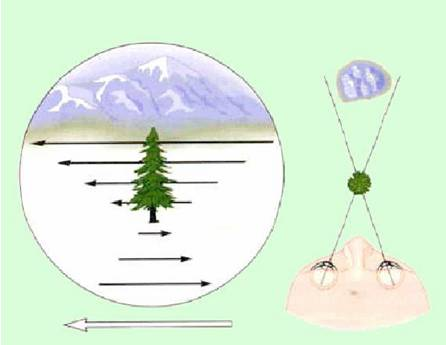
\includegraphics[width=0.7\linewidth]{figure/parallax}
					\caption{ [Copyright: \url{https://www.skybrary.aero/index.php/Vision_(OGHFA_BN)}]}
					\label{fig:parallax}
				\end{figure}
			\paragraph{Optic Flow}
				Image flying in space with a really fast space jet-pack, you just keep flying straight, with all the stars around you are whizzing by, except the point you are flying straight towards, the focus of expansion, isn't going anywhere. This cue is gotten from the relative motion from yourself and the scene you are moving around in, i.e. space. In \autoref{fig:opticFlow} is a visual representation of what it would look like to be in that really fast space jet-pack, with the focus of expansion being the middle point, and all the stars moving faster the closer they get to the edge of your periphery \citep{sensationPerception}.
				\begin{figure}[H]
					\centering
					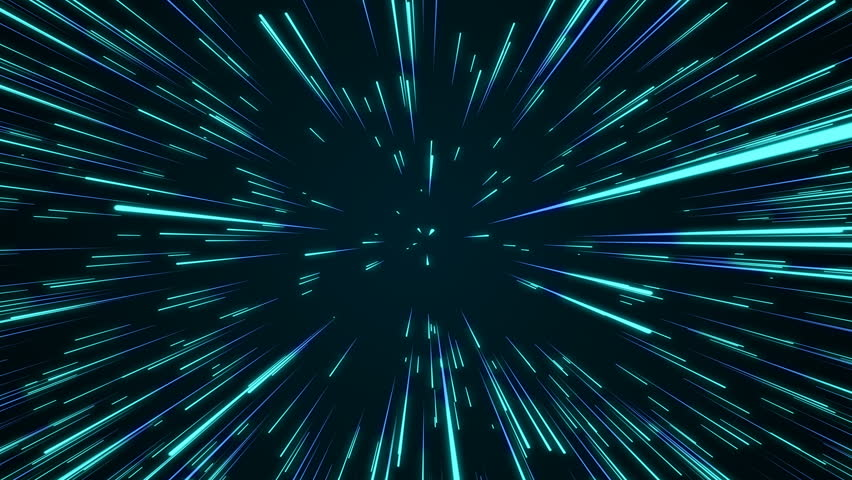
\includegraphics[width=0.7\linewidth]{figure/opticFlow}
					\caption{ [Copyright: shutterstock]}
					\label{fig:opticFlow}
				\end{figure}
			\paragraph{Deletion \& Accretion}
				A image that represents this cue very well can be found at \citep[p.~207]{sensationPerception}.
	
		\subsection{Stereopsis}
			The sense of depth, coming from having like two eyes and shit.
		\subsection{binocular disparity}
		Difference between the eyes and shit
		
		\subsection{Stereograms}
		Two images taken with approximately 6 cm (average distance between eyes) separation, produce the feel of depth in the person looking at it.
		
		\subsection{Autostereograms}
			Image that if viewed correctly looks like it has depth, many different versions.